\documentclass[a4paper]{scrartcl}

\usepackage[T1]{fontenc}
%\usepackage{wallpaper}
\usepackage{cook}

\newcommand\kochbuchauthor{Sebastian Preisner und Nicole Neumann}
\newcommand\kochbuchurl{http://www.calyrium.org/}
\newcommand\kochbuchtitle{Fitness Küche}
\newcommand\kochbuchversion{Ver. 0.3}

\newcommand{\caps}{www.calyrium.org}

\setcounter{secnumdepth}{-1} % um die nummerierung von sections zu unterbinden und trotzdem die PDF-Bookmarks zu haben

% Schriftarten fuer Ueberschriften
\usepackage{aurical}
\usepackage{calligra}
\usepackage{yfonts}
\usepackage{uncial}
\usepackage{rustic}
\usepackage{emerald}
%\usepackage{rotunda}
%\usepackage{inslrmin}
%\usepackage{pbsi}
%\usepackage{egothic}
%\usepackage{carolmin}
%%\usepackage{chancery}
%\usepackage{sqrcaps}


\definecolor{darkblue}{rgb}{0,0,.5}
\usepackage[ % muss letztes Package sein!
	pdftitle={\kochbuchtitle},%
	pdfauthor={\kochbuchauthor},%
	pdfsubject={Kochbuch},%
	pdfcreator={PDFLaTeX},
	colorlinks=true, urlcolor=darkblue, linkcolor=darkblue, bookmarksopen=true
 ]{hyperref} % 
%\twosided 	% Zweiseitig?

\usekomafont{section}
\addtokomafont{section}{\newpage\centering\vspace*{2cm}\rmfamily\Huge\color{darkred}}

%================== Symbolliste ====================
\usepackage{nomencl}

\makenomenclature


% ============================= Einheiten ==============================
\newcommand{\g}{\,g }
\newcommand{\kg}{\,kg }
\newcommand{\ml}{\,ml }
\renewcommand{\l}{\,l }
\newcommand{\TL}{\,TL }
\newcommand{\EL}{\,EL }
\newcommand{\cm}{\,cm }
\newcommand{\m}{\,m }
\renewcommand{\min}{\,min }
\newcommand{\pkg}{\,Päckchen}
\newcommand{\msp}{\,Msp.}

% ============================= Abkuerzungen ==============================
\newcommand{\bzw}{bzw.\@\xspace}
\newcommand{\bzgl}{bzgl.\@\xspace}
\newcommand{\ca}{ca.\@\xspace}
\newcommand{\dah}{d.\thinspace{}h.\@\xspace}
\newcommand{\Dah}{D.\thinspace{}h.\@\xspace}
\newcommand{\ds}{d.\thinspace{}sind\@\xspace}
\newcommand{\evtl}{evtl.\@\xspace}
\newcommand{\ua}{u.\thinspace{}a.\@\xspace}
\newcommand{\Ua}{U.\thinspace{}a.\@\xspace}
\newcommand{\usw}{usw.\@\xspace}
\newcommand{\va}{vor allem\@\xspace}
\newcommand{\vgl}{vgl.\@\xspace}
\newcommand{\zB}{z.\thinspace{}B.\@\xspace}
\newcommand{\ZB}{Zum Beispiel\xspace}
\newcommand{\sa}{s.\ auch\@\xspace}
\newcommand{\ia}{i.\thinspace{}Allg.\@\xspace}
\newcommand{\su}{s.\ unten\@\xspace}
\newcommand{\uvm}{u.\thinspace{}v.\thinspace{}m.\@\xspace}
\newcommand{\uva}{u.\thinspace{}v.\thinspace{}a.\@\xspace}
\newcommand{\uae}{u.\thinspace{}ä.\@\xspace}
\newcommand{\tk}{TK\@\xspace}

\begin{document}

% entweder die Optionen ausfüllen und mit \maketitle Titelseite erzeugen oder...
%\title{Meine Küche}
%\author{Autor}
%\maketitle

% ... die Titelseite selber zusammenstellen
\pdfbookmark[1]{Titel}{Meine Fitnessküche}
\begin{titlepage}
		\begin{center}
		\textcolor{white}{\\[4.5cm]\bfseries{	\scalebox{5.5}{Fitness} \\[1,5cm]\scalebox{5.5}{Küche} \\[1cm]\scalebox{1.2}{mit \arabic{recipes} Rezepten.}
				\\[12cm]\scalebox{1.8}{\kochbuchurl} } \\ \centering\vspace*{1cm}\copyright \ 2015 \kochbuchauthor \ \ \kochbuchversion}
		\end{center}
		\ThisCenterWallPaper{1}{./bilder/start2.jpg}
		%\begin{figure}[H]% einfügen der Grafik
			%\centering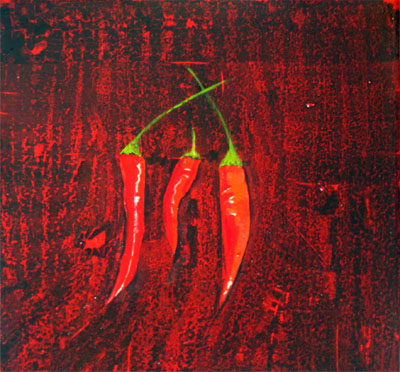
\includegraphics[width=0.95\textwidth]{./bilder/start2.jpg}
			%\centering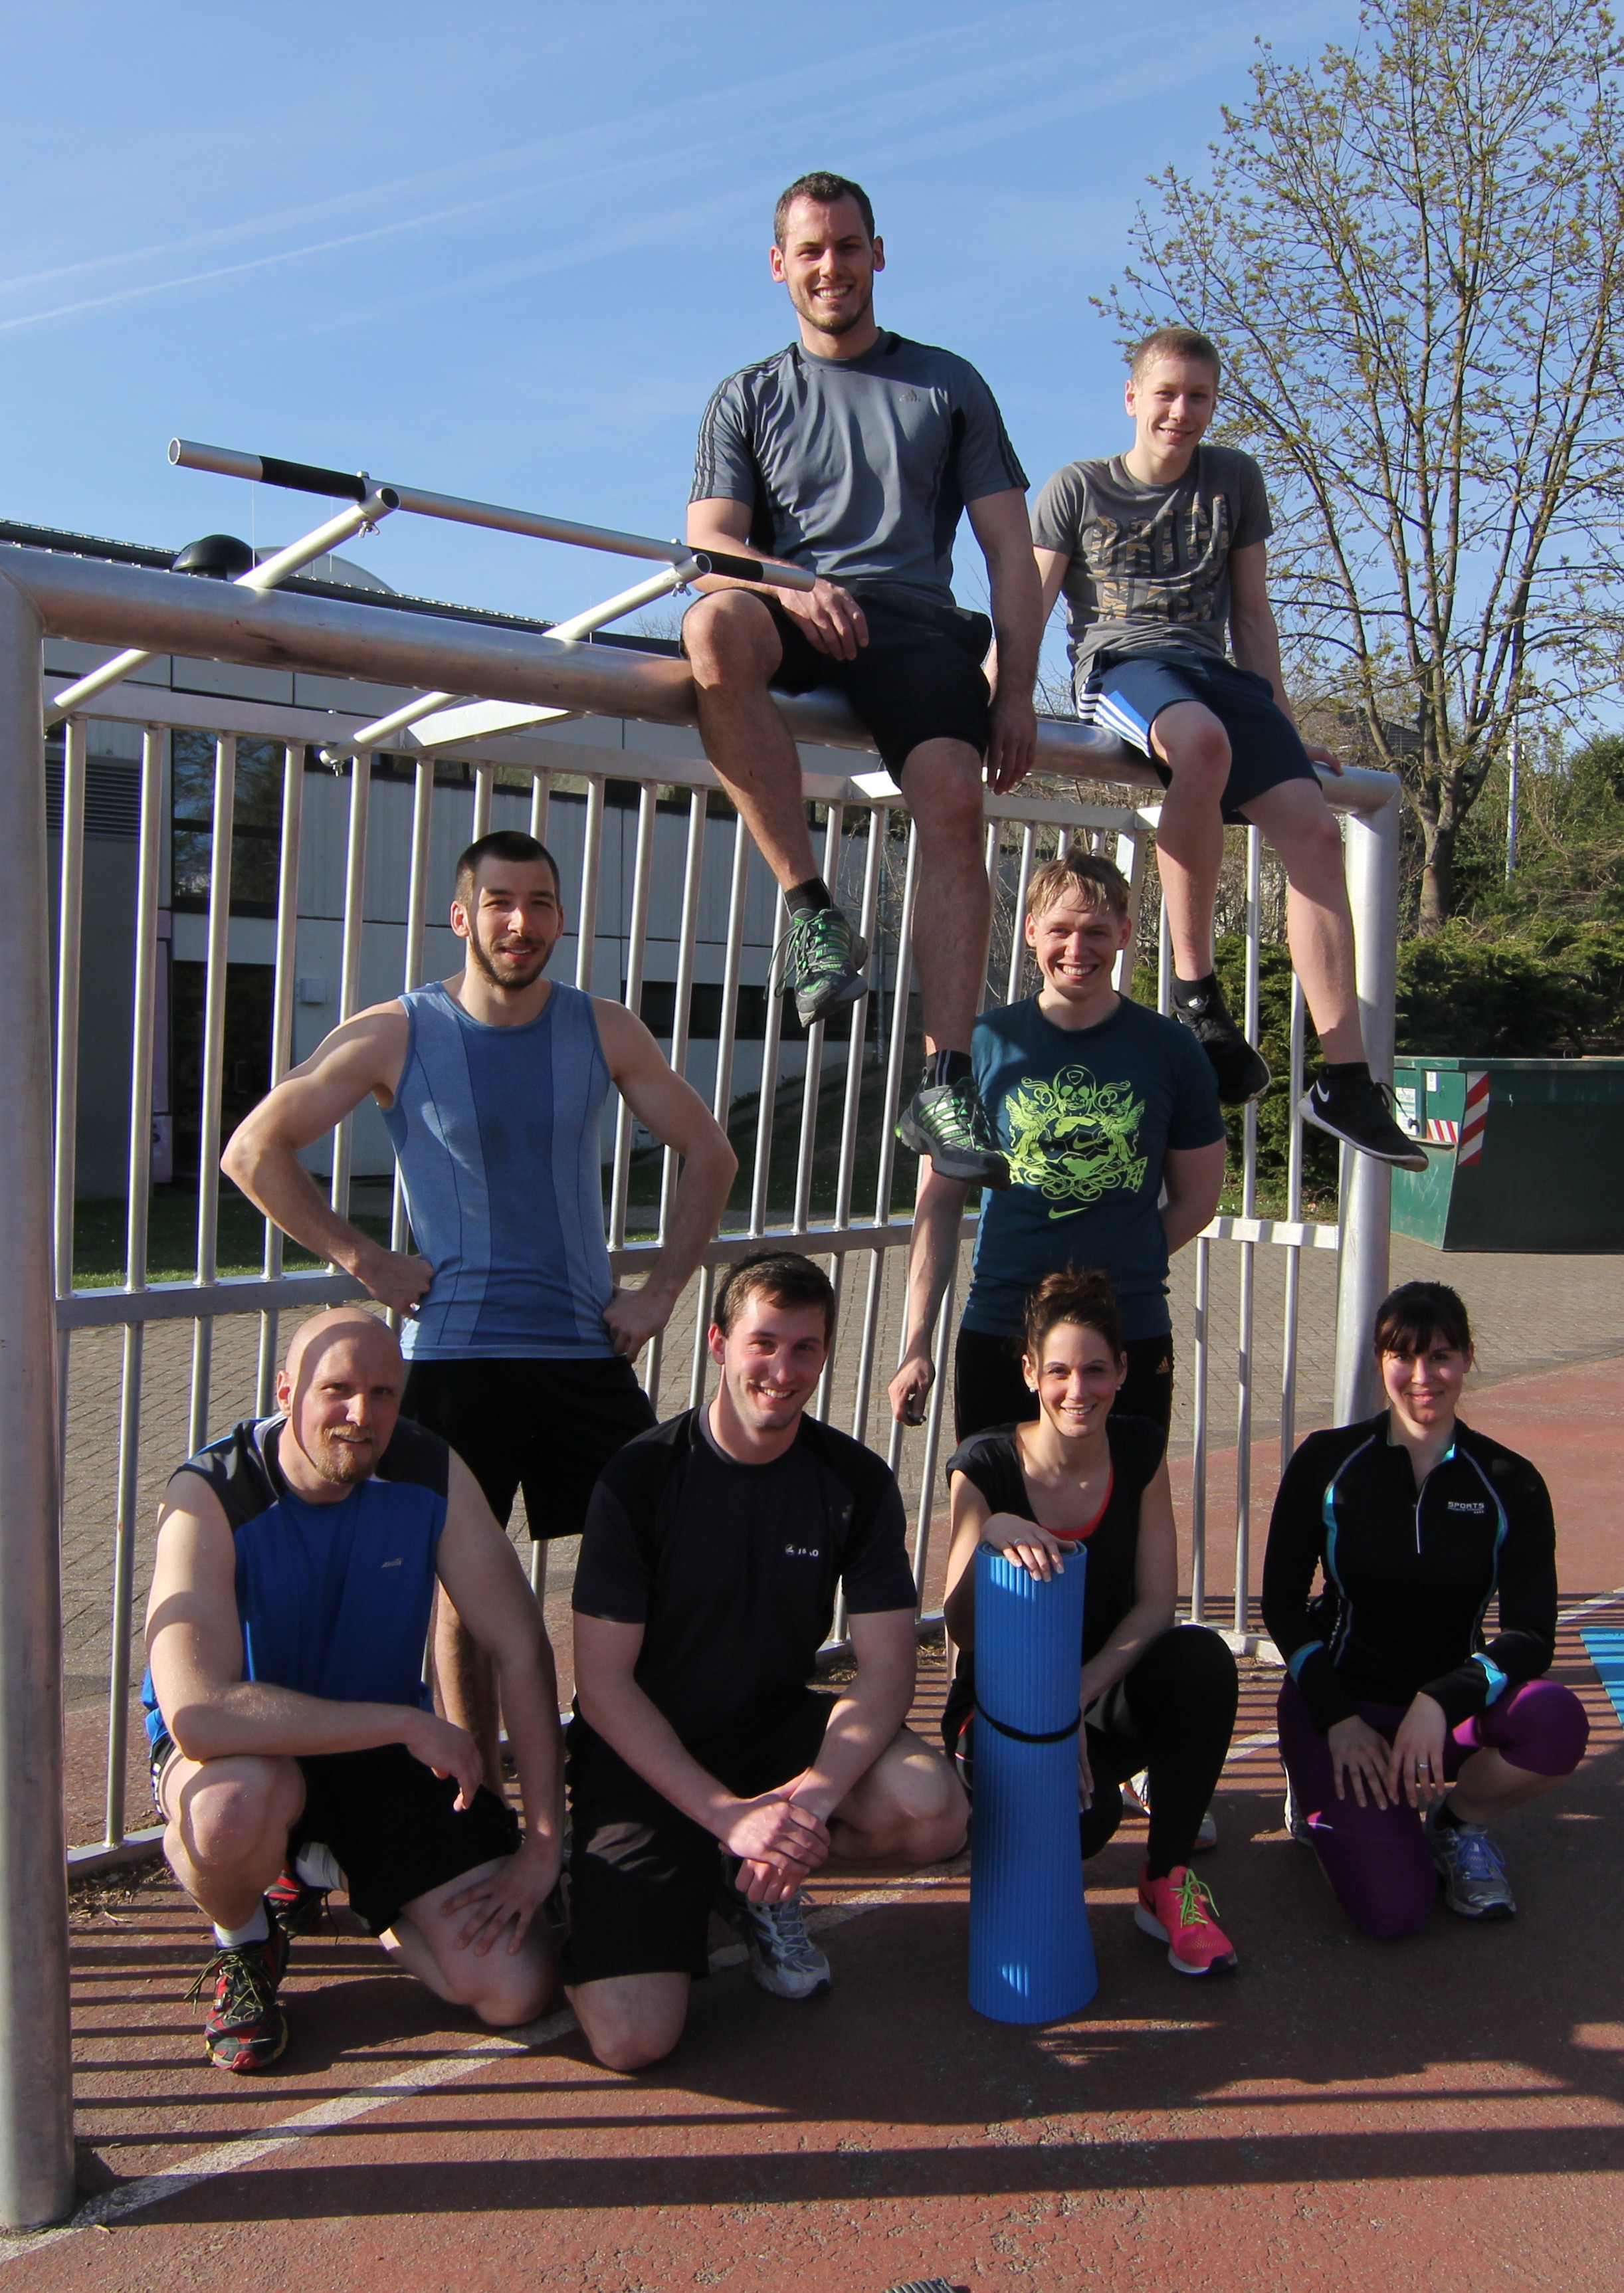
\includegraphics[height=0.94\textheight]{./bilder/start.jpg}
		%\end{figure}
\newpage
%\centering\vspace*{3cm}\copyright \ 2011 \kochbuchauthor
\end{titlepage}

\pdfbookmark[1]{Inhaltsverzeichnis}{toc}
\tableofcontents

% Standardfarbe, -schriftart für die Überschrift
\recipecolor{C08C23}

% Schriftart der Ueberschrift
%\recipefont{\rustfamily}
%\recipefont{\calligra}
%\recipefont{\Fontskrivan}
\recipefont{\Fontlukas}
%\recipefont{\Fontamici}
%\recipefont{\cminfamily}
%\recipefont{\rmfamily}
%\recipefont{\ECFJD}

% wenn \twosided aktiv ist (bei Zweiseitig ist die ungerade Zahl immer auf der Vorderseite)
% müssen hier soviele newpages einfügen bis die erste Sektion auf einer ungeraden Seite beginnt
\newpage~
\subsection*{\centering Danksagung}
\begin{quote}
Vielen Dank an \emph{Stefan Gabauer} der mit seinem Chili Cook Book\footnote{\url{http://sourceforge.net/projects/chilicookbook}} die \LaTeX-Stil-Vorlage von \emph{Christian Gatzlaff} zugänglich gemacht hat und uns somit das Werkzeug zur Erstellung dieses Fitnesskochbuchs in die Hand gegeben hat.\\

Wir möchten uns natürlich bei all den Kreativen Köpfen bedanken die ihre Rezeptideen mit uns geteilt haben und uns so zu dieser Zusammenstellung Inspiriert haben.
\vspace{2cm}

\subsection*{\centering Lizenz}
\begin{center}
"Fitness Küche"'\\
\textit{Dieses Kochbuch zeigt das gesunde Ernährung auch gut schmecken kann!}\\
Copyright (C) 2015 Sebastian Preisner\\

\begin{center}
	\href{http://creativecommons.org/licenses/by-nc-sa/3.0/de/}{
\includegraphics{cclogo.png}}
\end{center}

Fitness Küche von Sebastian Preisner und Nicole Neumann steht unter einer\\ \href{http://creativecommons.org/licenses/by/4.0/}{Creative Commons Namensnennung 4.0 International Lizenz.}\\
\url{http://creativecommons.org/licenses/by/4.0/}
\end{center}
\end{quote}

\newpage~
\subsection*{Einführung}
In dieser Rezeptsammlung haben wir die Rezepte zusammengestellt die uns besonders gut gefallen haben seit unserer Ernährungsumstellung. So entsteht ein Kochbuch für Ernährungsbewusste, Sportler und Menschen die nach neuen Ideen suchen. In diesem Projekt wird wert auf die Zubereitung und auf den Inhalt der Gerichte gelegt. Viele der Rezepte harmonieren nicht nur mit dem Ziel einer Ausgewogenen Ernährung sondern helfen auch beim Muskelaufbau und Fettabbau. 
Die Rezeptideen stammen aus Facebook, Youtube, Bücher und Webseiten und sind im Laufe unserer 
Ernährungsumstellung auf unsere Teller gekommen. Die Quelle eines jeden Rezeptes findet ihr am ende des Rezeptes, so könnt ihr über das Buch hinaus weitere Rezepte finden die zu euch und eurer Ernährung passen. 

Dieses Buch erhebt keinen Anspruch auf Perfektion, Korrektheit oder Vollständigkeit, es ist als kleine Rezeptsammlung für den privaten Gebrauch gedacht und wird je nach Zeit und Laune erweitert und verbessert.

\subsection*{Mitwirken}
Wir freuen uns immer über neue Rezeptideen und möchten natürlich das dieses Buch weiter wächst. Gerne kannst du dich daran beteiligen indem du uns dein Lieblingsrezept mitteilst. Dies geht entweder über Github\footnote{\url{https://github.com/kreativmonkey/Fitnesskueche}} oder aber auch per E-Mail (fitnesskueche@inmediato.de). 

\nomenclature{\Interval}{Zeitangabe der Zubereitung}%
\nomenclature{
\includegraphics[scale=0.40]{bilder/FEUER.png}}{Schärfegrad von 0-5}%
\nomenclature{$A$}{The area of the needle point}%
%Symbole ausgeben
\printnomenclature

%\Oven = Ofen
%\Topbottomheat = Ober- und Unterhitze
%\Topheat = Oberhitze
%\Bottomheat = Unterhitze
%\Fanoven = Umluft
%\Gasstove = Gasofen
%\Dish = Teller (Angabe der Portionen)
%\Knife = Messer
%\Fork = Gabel
%\Spoon = Löffel
%\Gloves = Handschuhe
%
\includegraphics[scale=0.40]{bilder/FEUER.png} = Schärfe von 1 bis 5

%%%%%%%%%%%%%%%%%%%%%%%%%%%%%%%%%%%%%%%%%%%%%%%%%%%%%%%%%%%%%%%%%%%%%%%%%%%%%%%%%%%%%%%%%%%%%%%

\section{Basic} %%%%%%%%%%%%%%%%%%%%%%%%%%%%%%%%% Konservieren
% ====== Rezeptname und die Quelle ======
\begin{recipe}[]{ Falscher Reis }{ Chefkoch: http://www.chefkoch.de/rezepte/2506181393345016/Falscher-Reis.html }{  }

Falscher Reis besteht aus Blumenkohl und zeichnet sich durch seinen geringen Kohlenhydratanteil aus. Er eignet sich gut als Beilage und kann wie Reis verwendet werden.

% ====== Zeit, Personen und Schärfe ======
%\timerecipe{ca. 1}         % Zubereitungszeit in Stunden
\timerecipe[Minuten]{15}    % oder in Minuten
\personcount{2}        		% Personenanzahl
\spicecount{0}              % Schaerfe von 5

% ====== Zutaten ======
\ingredient{700\g Blumenkohl}
\ingredient{2\EL Butter}
\ingredient{1 Prise Salz}
\ingredient{etwas Muskat}

% ====== Zubereitung ======    
\step
Den gewaschenen Blumenkohl in Röschen zerteilen und in einen Mixer geben. Vorsichtig auf höchster Stufe die Röschen zerkleinern, so das sie die Größe von Reiskörner bekommen. Darauf achten das es nicht mußig wird. 

\step
Die Blumenkohlreiskörner in ein Mikrowellen geeignetes Gefäß geben und abgedeckt etwa 5-8 Minuten (je nach Leistung) in der Mikrowelle garen. Nach der Hälfte einmal kurz durchschütteln.

\step
Nach dem Garen mit Butter, Salz und Muskatnuss abschmecken.

% Tipp in extra Rahmen mit dem Wort "Tipp:" am Anfang
\tippboxtip{Passt besonders gut zu Gerichten mit viel Soße.} 

         % ====== Bild ======
% Grafik fuer das Rezept koennen so eingefuegt werden:
% wenn kein Bild vorhanden ist, bitte diese Zeile auskommentiert lassen.
%\graphic{./bilder/todo.jpg}
\end{recipe}
% ====== Rezeptname und die Quelle ======
\begin{recipe}[]{ Fitness Mayonnaise }{ http://eatsmarter.de/rezepte/leichte-mayonnaise }{  }

% ====== Zeit, Personen und Schärfe ======
\timerecipe{ca. 7}         % Zubereitungszeit in Stunden
%\timerecipe[Minuten]{10}    % oder in Minuten
\personcount{4}        		% Personenanzahl
\spicecount{0}              % Schaerfe von 5

% ====== Zutaten ======
\ingredient{200\g Magerquark}
\ingredient{4 Eier}
\ingredient{\sfrac{1}{2} Zitrone}
\ingredient{1\EL Weißweinessig}
\ingredient{1-2\EL Wasser}
\ingredient{1\msp Cayennepfeffer}
\ingredient{Salz}

% ====== Zubereitung ======    
\step
Den Quark in einem feinen Sieb ca. 4 Stunden abtropfen lassen.

\step
Die Eier in einem kleinen Topf mit Wasser bedecken und zum Kochen bringen. Genau 9 Minuten kochen und unter kaltem Wasser abschrecken. Danach werden die Eier gepellen und halbiert und das Eigelb mit einem Teelöffel herausgelöst.  

\tippbox{Eiweiße anderweitig verwenden, z. B. hacken und über einen Salat streuen.}

\step
Das Wasser zum Eigelb geben und mit einem Holzlöffel zu einer cremigen Masse zerdrücken. Den Cayennepfeffer hinzugeben und nach und nach den abgetropften Quark unterrühren.

\step
Die Zitrone auspressen und 1-2\TL vom Saft mit dem Essig unter die Quarkeimasse mischen. 

\step 
Die fertige Masse nun noch 2-3 Stunden kalt stellen und genießen.

% Tipp in extra Rahmen mit dem Wort "Tipp:" am Anfang
%\tippboxtip{ } 

         % ====== Bild ======
% Grafik fuer das Rezept koennen so eingefuegt werden:
% wenn kein Bild vorhanden ist, bitte diese Zeile auskommentiert lassen.
%\graphic{./bilder/todo.jpg}
\end{recipe}
% ====== Rezeptname und die Quelle ======
\begin{recipe}[]{ Rapsöl Mayo }{ Moin Yamina auf \href{https://www.youtube.com/watch?v=I68KLKFsKpM}{Youtube} }{  }

% ====== Zeit, Personen und Schärfe ======
%\timerecipe{ca. 4}         % Zubereitungszeit in Stunden
\timerecipe[Minuten]{5}    % oder in Minuten
\personcount{2}        		% Personenanzahl
\spicecount{0}              % Schaerfe von 5

% ====== Zutaten ======
\ingredient{2 Eigelb}
\ingredient{1\sfrac{1}{2}\EL Senf}
\ingredient{6\EL Rapsöl}
\ingredient{3\EL Wasser}
\ingredient{große \pr Salz}

% ====== Zubereitung ======
\step
Alle Zutaten in einen Mixbehälter geben und gut vermischen.


% Tipp in extra Rahmen mit dem Wort "Tipp:" am Anfang
\tippboxtip{Eignet sich gut als Sauce zu Backofenkartoffeln.}

         % ====== Bild ======
% Grafik fuer das Rezept koennen so eingefuegt werden:
% wenn kein Bild vorhanden ist, bitte diese Zeile auskommentiert lassen.
%\graphic{./bilder/todo.jpg}
\end{recipe}

%\input{./rezepte/pommesvariationen.tex}


%\section{Frühstück} %%%%%%%%%%%%%%%%%%%%%%%%%%%%%%%%% Konservieren


%\section{Suppen} %%%%%%%%%%%%%%%%%%%%%%%%%%%%%%%% Suppen


%\section{Salate} %%%%%%%%%%%%%%%%%%%%%%%%%%%%%%%% Salate


\section{Hauptgerichte} %%%%%%%%%%%%%%%%%%%%%%%%%%%%%%%% Hauptgerichte
% ====== Rezeptname und die Quelle ======
\begin{recipe}[]{ Thunfischfrikadellen mit Asia-Salat }{ Freeletics Ernährungsguid }

% ====== Zeit, Personen und Schärfe ======
%\timerecipe{ca. 1}         % Zubereitungszeit in Stunden
\timerecipe[Minuten]{15}    % oder in Minuten
\personcount{1}        		% Personenanzahl
\spicecount{0}              % Schaerfe von 5

% ====== Zutaten ======
\ingredient{150\g Thunfisch in der Dose}
\ingredient{30\g Haferflocken oder Hafermehl}
\ingredient{1 Ei}
\ingredient{1/2 Zwiebel}
\ingredient{1 Pak Choi (\ca 200\g)}
\ingredient{1 Frühlingszwiebel}
\ingredient{100\g Soja- oder Mungobohnensprossen}
\ingredient{2 \EL Sesam (\ca 20\g)}
\ingredient{1 daumengroßes Stück Ingwer}
\ingredient{1/2 Limette}
\ingredient{3 \EL Sojasauce}

         % ====== Zubereitung ======    
\step
Den Thunfisch mit einer Gabel zerpflücken. Haferflocken in einem Mixer auf höchster Stufe zu einer Art Mehl verarbeiten. Zwiebeln abziehen und klein schneiden. Den Sesam währenddessen in einer Pfanne ohne Fett auf mittlerer Hitze \ca 3 Minuten anrösten. 

\step
Thunfisch, Haferflocken, Ei und Zwiebelwürfel gründlich vermengen. Aus der so entstehenden Masse werden nun 4 gleichgroße Frikadellen geformt. 

\step 
Öl in einer Pfanne bei mittlerer Hitze heiß werden lassen und die Thunfischfrikadellen von jeder Seite \ca 4 Minuten braten.\\ 
Währenddessen Pak Choi, Paprika, Frühlingszwiebel und -falls nötig- Sprossen waschen, trocken tupfen.

\tippbox{Frische Sprossen schmecken einfach am besten. Gibt es oft in großen Supermärkten zu erwerben oder beim Asialaden um die Ecke.}

\step
Pak Choi und Paprika in Streifen schneiden, Frühlingszwiebel in Ringe schneiden und mit den Sprossen und dem Sesam mischen. 

\step 
Den Ingwer nach dem schälen auf einer Reibe fein raspeln und zusammen mit dem Saft der ausgepressten Limette und der Sojasauce auf den Salat geben.

\tippboxtip{Dies ist ein umrahmter Tipp um noch ein paar Zusatzinformationen und weitere Anregungen dem Rezept beizufügen.} 
% Tipp in extra Rahmen mit dem Wort "Tipp:" am Anfang

         % ====== Bild ======
% Grafik fuer das Rezept koennen so eingefuegt werden:
% wenn kein Bild vorhanden ist, bitte diese Zeile auskommentiert lassen.
%\graphic{./bilder/todo.jpg}
\end{recipe}
% ====== Rezeptname und die Quelle ======
\begin{recipe}[]{ Putenbruststreifen mit Erdnusschilisauce }{ Freeletics Nutrationguid }

% ====== Zeit, Personen und Schärfe ======
%\timerecipe{ca. 1}         % Zubereitungszeit in Stunden
\timerecipe[Minuten]{35}    % oder in Minuten
\personcount{2}        		% Personenanzahl
\spicecount{1}              % Schaerfe von 5

% ====== Zutaten ======
\ingredient{400\g Puten- oder Hänchenbrustfilet}
\ingredient{300\g Blumenkohl}
\ingredient{100\g Lauch}
\ingredient{4 Möhren}
\ingredient{200\ml Kokosmilch (ungesüßt)}
\ingredient{8\EL Erdnussbutter (ungesüßt)}
\ingredient{2 Knoblauchzehe}
\ingredient{2 daumengroße Stück Ingwer (40\g)}
\ingredient{1 Limette}
\ingredient{1\TL Chilliflocken oder -ringe}
\ingredient{4\TL Raps- oder Olivenöl}
\ingredient{Salz, Pfeffer}

         % ====== Zubereitung ======    
\step
Puten- oder Hänchenbrustfilet mit kalten Wasser abbrausen, trockentupfen und in \ca 1\cm dicke Streifen schneiden. Den Blumenkohl in Scheiben schneiden. Den Lauch waschen, trockentupfen und in Scheiben schneiden. Möhren schälen und in Scheiben schneiden.
 
\step
In einer Pfanne auf mittlerer Hitze 2\TL Olivenöl erhitzen und darin die Filetstreifen und das Gemüse \ca 2 Minuten von jeder Seite anbraten. Das Fleisch herausnehmen und beiseite legen. 150\ml Wasser auf das Gemüse geben und köcheln lassen bis das Wasser verdampft ist (\ca 5 \min)
\tippbox{Das Fleisch auf einem im Backofen vorgeheizten Teller bei 50 Grad in den Backofen.}

\step
Für die Sauce den Knoblauch und Ingwer schälen und in dünne Scheiben schneiden. Die Zitrone/Limette halbieren und auspressen. In einem Topf bei mittlerer Hitze 1\TL Olivenöl heiß werden lassen und den Knoblauch, Ingwer und die Cihili \ca 3 \min anbraten.

\step
Die Sauce mit Kokosmilch ablöschen, kurz aufkochen lassen und dann vom Herd nehmen. Nun wird die Erdnusscreme und der Limettensaft eingerührt, danach mit Salz und Pfeffer abschmecken.

\step
Putenstreifen mit Gemüse und Erdnusssauce anrichten und  genießen.

% Tipp in extra Rahmen mit dem Wort "Tipp:" am Anfang
\tippboxtip{Dies ist ein umrahmter Tipp um noch ein paar Zusatzinformationen und weitere Anregungen dem Rezept beizufügen.} 

         % ====== Bild ======
% Grafik fuer das Rezept koennen so eingefuegt werden:
% wenn kein Bild vorhanden ist, bitte diese Zeile auskommentiert lassen.
\graphic{./bilder/Putenstreifen_mit_Erdnusschilisauce.jpg}
\end{recipe}
% ====== Rezeptname und die Quelle ======
\begin{recipe}[]{ Veggie Burger }{ }{  }

% ====== Zeit, Personen und Schärfe ======
\timerecipe{ca. 40}         % Zubereitungszeit in Stunden
%\timerecipe[Minuten]{10}    % oder in Minuten
\personcount{4}        		% Personenanzahl
\spicecount{0}              % Schaerfe von 5

% ====== Zutaten ======
\ingredient{150\g Champignons}
\ingredient{425\g rote Kidneybohnen}
\ingredient{1 Knoblauchzehe}
\ingredient{1 Zwiebel}
\ingredient{1\TL gemahlener Koriander}
\ingredient{1\TL gemahlener Kreutzkümmel}
\ingredient{2\EL glatte Petersilie, frisch gehackt}
\ingredient{1\EL Oliven-/Rapsöl}
\ingredient{Salz, Pfeffer}
\ingredient{Mehl}
\ingredient{1 Ei}

% ====== Zubereitung ======    
\step
Knoplauch, Zwiebel und Champignons fein hacken. In einer Pfanne das Öl erhitzen und die Zwiebeln für 5 Minuten weich dünsten. Danach den Koriander, Kreuzkümmel und den Knoblauch zugeben und unter gelegentlichem Rühren 1 Minute dünsten. Nun die Pilze zugeben und für 5 Minuten garen.

\step
Währenddessen die Bohnen abtropfen und abspülen und danach in einer Schüssel mit einem Kartoffelstampfer oder einer Gabel zerdrücken. Die Petersilie hinzugeben und verrühren.

\tippbox{Gib an dieser Stelle ein Ei hinzu damit die Masse besser zusammenhält. Es geht jedoch auch ohne Ei}

\step
Die Pilzmischung zu den Bohnen hinzugeben und gut Mischen. 

\step 
Die Masse in 4 Portionen aufteilen und in etwas Mehl wenden. Die Teile zu flachen, runden Burgern formen und mit Öl bestreichen.

\step 
Die Taler auf einem Blech verteilen und in den Vorgeheizten Backofen (Grill oder 200 Grad Oberhitze) für 5-7 Minuten von jeder Seite grillen.

\tippbox{ Funktioniert auch in der Pfanne. }

% Tipp in extra Rahmen mit dem Wort "Tipp:" am Anfang
\tippboxtip{Variation: Die Pilze lassen sich auch Prima durch eine Zucchini-Karotten Mischung ersetzen.} 

         % ====== Bild ======
% Grafik fuer das Rezept koennen so eingefuegt werden:
% wenn kein Bild vorhanden ist, bitte diese Zeile auskommentiert lassen.
%\graphic{./bilder/todo.jpg}
\end{recipe}

%\section{Saucen} %%%%%%%%%%%%%%%%%%%%%%%%%%%%%%%%%%%%%%% Soucen


%\section{Snaks} %%%%%%%%%%%%%%%%%%%%%%%%%%%%%%%% Snaks


\section{Süße Snaks} %%%%%%%%%%%%%%%%%%%%%%%%%%%%%%%% Süßes
% ====== Rezeptname und die Quelle ======
\begin{recipe}[]{ Brownie Delux }{ \href{https://www.youtube.com/channel/UCR_dfR8wJBmsVkQFDa3PDcQ}{Moin Yamina auf Youtube} }

% ====== Zeit, Personen und Schärfe ======
%\timerecipe{ca. 1}         % Zubereitungszeit in Stunden
\timerecipe[Minuten]{10}    % oder in Minuten
%\personcount{4}        		% Personenanzahl
%\spicecount{3}              % Schaerfe von 5

% ====== Zutaten ======
\ingredient{200\g gemahlene Mandeln}
\ingredient{200\g Kakao}
\ingredient{250\g getrocknete Datteln}
\ingredient{1 Schuss Rum}
\ingredient{Wasser nach bedarf}

         % ====== Zubereitung ======    
\step
Die Datteln mit einem Mixer oder Zauberstab und dem Schuss Rum zerkleinern. Je nach bedarf Wasser hinzufügen bis die Datteln zu einer einheitlichen cremigen Masse werden.

\step
Die gemahlenen Mandeln und den Kakao vermischen und die Dattelmasse hinzufügen. Alles gut vermengen.

\tippbox{Mit einem Löffel habe ich die beste Erfahrung gemacht. Mit den Händen geht es auch und man hat sehr viel zu naschen ;-).}

\step
Die fertige Masse auf einem Backpapier oder Brotpapier verteilen und zu einem flachen Kasten formen. Fertig.

\tippboxtip{Das Rezept kann mit belieben abgewandelt werden. \zB kann man die Masse zu Kugeln formen und mit Haselnüssen füllen. Lass deiner Phantasie freien lauf.} 
% Tipp in extra Rahmen mit dem Wort "Tipp:" am Anfang

         % ====== Bild ======
% Grafik fuer das Rezept koennen so eingefuegt werden:
% wenn kein Bild vorhanden ist, bitte diese Zeile auskommentiert lassen.
%\graphic{./bilder/todo.jpg}
\end{recipe}
% ====== Rezeptname und die Quelle ======
\begin{recipe}[]{ Himbeer-Muffins }{\href{http://www.lowcarb-ernaehrung.info/rezept-kokos-himbeer-muffins/}{http://www.lowcarb-ernaehrung.info/rezept-kokos-himbeer-muffins/}}{ }

% ====== Zeit, Personen und Schärfe ======
%\timerecipe{ca. 1}         % Zubereitungszeit in Stunden
\timerecipe[Minuten]{10}    % oder in Minuten
\personcount{4}        		% Personenanzahl
\spicecount{0}              % Schaerfe von 5

% ====== Zutaten ======
\ingredient{3 Eier}
\ingredient{\sfrac{1}{4} Tasse geschmolzene Butter}
\ingredient{\sfrac{1}{4} Tasse Zuckeraustauschstoff (nach belieben)}
\ingredient{\sfrac{1}{3} Tasse Kokosnussmehl}
\ingredient{\sfrac{1}{2} Tasse Himbeeren, Blaubeeren oder Beerenmix}
\ingredient{\sfrac{1}{2}\TL Backpulver}
\ingredient{\sfrac{1}{2}\TL Vanille}
\ingredient{1 Prise Salz}
\ingredient{2-5\EL Wasser}

% ====== Zubereitung ======    
\step
Den Backofen auf 190 Grad vorheizen. Währenddessen die Eier verquierlen. Nach und nach die geschmolzene Butter, die Vanille, das Salz sowie den Zuckeraustauschstoff zu den Eiern hinzugeben. Anschließend das Kokosnussmehl sowie Backpulver zufügen. Den Teig so lange verrühren bis eine glatte Masse entsteht. 

\tippbox{Je nach Konsistenz des Teiges etwas Wasser beimischen. Der Teig sollte nicht zu dick aber auch nicht zu dünn sein.}

\step
Die Beeren unter den Teig heben und dann in die Muffinformen. Die Muffins für 15 bis 20 Minuten in den Backofen geben bis sie gold-braun sind. 

% Tipp in extra Rahmen und mit Hintergrundfarbe sowie dem Wort "Tipp:" am Anfang
%\tippboxtip{Dies ist ein umrahmter Tipp um noch ein paar Zusatzinformationen und weitere Anregungen dem Rezept beizufügen.} 

         % ====== Bild ======
% Grafik fuer das Rezept koennen so eingefuegt werden:
% wenn kein Bild vorhanden ist, bitte diese Zeile auskommentiert lassen.
%\graphic{./bilder/todo.jpg}
\end{recipe}
% ====== Rezeptname und die Quelle ======
\begin{recipe}[]{ Bananen Pancakes }{ \href{http://de.myprotein.com/thezone/rezepte/rezept-bananen-protein-pancakes/} }{  }

% ====== Zeit, Personen und Schärfe ======
%\timerecipe{ca. }         % Zubereitungszeit in Stunden
\timerecipe[Minuten]{10}    % oder in Minuten
\personcount{1}        		% Personenanzahl
\spicecount{0}              % Schaerfe von 5

% ====== Zutaten ======
\ingredient{1 Banane}
\ingredient{2 Eier}
\textbf{nach belieben:}
\ingredient{}
\ingredient{20\g Eiweißpulver}
\ingredient{1 Schuss Wasser/Milch}

% ====== Zubereitung ======    
\step
Die Banane in einer Schüssel zerdrücken und mit den Eiern (und Eiweißpulver) vermischen. Wenn das Gemisch zu dickflüssig wird mit etwas Wasser oder Milch verdünnen.

\step
In einer beschichteten Pfanne goldbraun braten und genießen.

\step 
\textbf{Toppings:} Mit Beeren, Sahne oder Ahornsirup, der Phantasie sind keine Grenzen gesetzt.

% Tipp in extra Rahmen mit dem Wort "Tipp:" am Anfang
\tippboxvar{Der Teig kann auch mit Zimt gewürzt werden.} 

         % ====== Bild ======
% Grafik fuer das Rezept koennen so eingefuegt werden:
% wenn kein Bild vorhanden ist, bitte diese Zeile auskommentiert lassen.
%\graphic{./bilder/todo.jpg}
\end{recipe}

%\section{Getränke} %%%%%%%%%%%%%%%%%%%%%%%%%%%%%%%%%%%%%%%% Getränke


\section{Smoothies} %%%%%%%%%%%%%%%%%%%%%%%%%%%%%%%%%%%%%%%% Smoothies
% ====== Rezeptname und die Quelle ======
\begin{recipe}[]{ Afterworkout-Beerenmix }{}{}

Dieser Shake zeichnet sich durch den hohen Eiweißgehalt aus und dient so als potentielle Eiweißquelle für nach dem Training, aber auch zur Erfrischung an Warmen Tagen kann der Trink gemacht werden.
% ====== Zeit, Personen und Schärfe ======
%\timerecipe{ca. 1}         % Zubereitungszeit in Stunden
\timerecipe[Minuten]{5}    % oder in Minuten
\personcount{1}        		% Personenanzahl
\spicecount{0}              % Schaerfe von 5

% ====== Zutaten ======
\ingredient{150\g \tk Beerenmix}
\ingredient{500\g Magerquark}
\ingredient{150\ml Wasser}
\ingredient{1 Vanilleschote}


         % ====== Zubereitung ======    
\step
Die Beeren zusammen mit dem Magerquark und dem Wasser in einem Mixer bei höchster Stufe \ca 1\min mixen.

\step
Die Vanilleschote mit einem Messer vorsichtig einschneiden und öffnen. Mit dem Messerrücken die Schote auskratzen und den Inhalt in den Mixer geben. Alles kurz durchmischen und fertig ist der Shake.

\tippboxtip{Dieses Rezept ist als Grundlage zu verstehen. Durch das verändern der Zutaten entstehen immer neue Geschmacksrichtungen. Probiere es aus. } 
% Tipp in extra Rahmen mit dem Wort "Tipp:" am Anfang

         % ====== Bild ======
% Grafik fuer das Rezept koennen so eingefuegt werden:
% wenn kein Bild vorhanden ist, bitte diese Zeile auskommentiert lassen.
%\graphic{./bilder/todo.jpg}
\end{recipe}

\section{Infos und Wissenswertes} %%%%%%%%%%%%%%%%%%%%%%%%%%%%%%%%%%%%%%%%% Info
\arabic{recipes}
	
%\end{itemize}

%%%%%%%%%%%%%%%%%%%%%%%%%%%%%%%%%%%%%%%%%%%%%%%%%%%%%%%%%%%%%%%%%%%%%%%%%%%%%%%%%%%%%%%%%%%%%%%
\end{document}